On peut modéliser la laine par une longue chaîne de $N \gg 1$ molécules identiques, que l'on suppose discernables et indépendantes les unes des autres. Une telle chaîne est appelée macromolécule ou polymère. Chaque molécule (ou monomère) peut se trouver
dans deux états notés $1$ et $2$ (voir figure). Dans l’état $1$, la molécule contribue pour $a$ à la longueur de la
chaîne et son énergie est $\epsilon_{a}$. Dans l’état $2$, sa longueur est $b$ et son énergie $\epsilon_{b}$. La chaîne est
soumise à une tension $F$ et est en équilibre avec un thermostat à la température $T$. L'énergie de la chaîne s'écrit dans ces conditions $E=\sum_{i=1}^{N} \epsilon_i-F\sum_{i=1}^{N} l_i$ où $l_i=a$ ou $b$ et $\epsilon_i=\epsilon_{a}$ ou $\epsilon_{b}$ selon la conformation $1$ ou $2$ du monomère $i$. {\bf On notera que $\bf a > b$}. Pour le calcul des ordres de
grandeur, on prendra $a = 2b = 2$ nm et $N = 10^4$.

\ 

\centerline{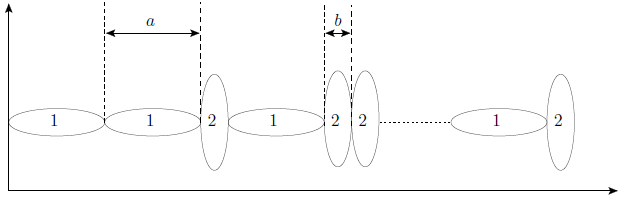
\includegraphics[height=.17\textwidth]{../Fig/keratine}}

\question Calculer la fonction de partition de la chaîne. 

\question En déduire son énergie moyenne $\overline{E}$ et sa longueur moyenne $\overline{L}$ à l'équilibre en fonction de $F$ et $T$.

On se place maintenant dans l'approximation où $\epsilon_{a} \approx \epsilon_{b}$.

\question Simplifier les expressions obtenues dans les questions ci-dessus.

\question \'Etudier, pour $F$ donnée, les limites basse température et haute température  de $\overline{E}$ et de $\overline{L}$. Interpréter les résultats.

\question Donner l'allure de la courbe $\overline{l}=\frac{\overline{L}}{N}$ en fonction de $F$ à $T$ donnée. Comment dans le cas des grandes forces $\beta F (a-b) \gg 1$, la limite asymptotique est-elle approchée ?

\question Montrer que dans le domaine des faibles forces, la chaîne vérifie la loi $F=K(T) (\overline{L} - L_0)$. Déterminer et interprétér $K(T)$ et $L_0$. Comment s'appelle cette loi ? Donner l'ordre de grandeur à température ambiante pour ces deux paramètres.

\question Peut-on en conclure quelque chose sur le lavage de la laine ?
